%-----------------------------------------%
\section{アバポンヌフ船長の文化的側面}
%-----------------------------------------%
\subsection{アボンポンヌ船長}
本研究グループは、アバポンヌ船長に対する研究を進めてきた。
アバポンヌ船長とは、その名の通り「船長」であり、様々な理論から存在が確実視されている船長人間である。
ここで船長人間とは船長でありながら人間である二重性を実現している存在であり、
前期量子力学的には光が粒子性と波動性の二重性を持っていると結論付けられたことの
類推によって理解することが可能となる。
しかし、「アバポンヌ」の部分に関しては様々な理論的予測は未だ乱立した状態にあり、
革新的・統一的な見解は得られていない。
アバポンヌは過去300年間未解明の現象であり、アバポンヌ問題が解けた場合、すべての物理事象を
描像することのできる大アバポンヌ1000元連立300次元方程式を導くことができる。
この超多次元連立方程式は現在のスーパーコンピューターの性能では、人類の有史と同じ程の
計算時間を要するため、アバポンヌ問題を解き連立方程式を導いても結局は何も言っていないのと
同義であるという至極真っ当な意見も多数見受けられる。\par

しかし、本研究グループでは別途スーパーハイパーコンピューターを開発したのでアバポンヌ連立方程式が導けた場合、そこから一般解は1秒で導出できると予測している。
そこで本研究グループでは数あるアバポンヌ理論のうち最も欠陥の少ない、ジェネラルアバポンヌ
理論を参考に解析を進めた。

%------------------------------------------%
\subsubsection{一般的な船長という概念}
%------------------------------------------%
本研究グループはアバポンヌ船長を研究対象にするために、まず一般的な船長という概念についての基礎研究を行った。\par
船長とは、特定の船舶の乗組員で、船舶の指揮者であるとともに船主(船舶所有者)の代理人として、乗組員の監督,船舶・積み荷の管理,運航の指揮などについて、
法律上多くの権限と義務を有している。
つまり船長とはその名の通り「船の長」であり、村長\footnote{アンゴラ村長を除く。}に匹敵する長である。
本研究グループは一般的な船長の持つ権限はアバポンヌ船長にも付与されているとする仮定(ジェネラルアバポンヌ仮定)を採用した。
この仮定はアバポンヌ船長の研究を進めている学会である船長学会において一般的に認知されている論法である。
以下に一般的な船長の有する権利をジェネラルアバポンヌ仮定で解釈を行った結果を列挙する。

\begin{description}
\item[(1)指揮命令権(船員法第7条)]\mbox{}\\
アバポンヌ船長は、理学部内での船長以外の教務委員(海員)を指揮監督し、かつ理学部(以下では船内)にある旅客などに対し、その職務を行うにつき必要な命令をすることができる。
その必要な命令は法律の範疇を超えることができ、軍司令部を掌握し理学部構内に戒厳令を敷くことも可能となり、対アバポンヌ船長の勢力への全面戦争の体勢は整っている。

\item[(2)懲戒権(船員法第22条)]\mbox{}\\
アバポンヌ船長は、船内規律を守らない海員を懲戒することができる。

\item[(3)強制権(船員法第25~28条)]\mbox{}\\
船長は、海員、旅客などが、凶器、爆発又は発火しやすい物、劇薬その他の危険物を所持するときは、その物につき保管、放棄などの必要な処置をすることができる。
つまり4年生実験の総指揮は実はアバポンヌ船長が執っており、何か問題があった場合理学部物理学科、化学科、生物学科、地球惑星学科の各専攻長はアバポンヌ船長への連絡が義務付けられている。
また、船内にある者の生命、身体又は船舶に危害を及ぼすような行為をしようとする海員その他船内にある者に対し、その危害を避けるのに必要な処置をすることができる。
船長は、海員が雇入契約の終了の公認があった後船舶を去らないときは、その海員を強制して船舶を去らせることができる。

\item[(4)行政庁に対する援助の請求(船員法第29条)]\mbox{}\\
船長は、海員・旅客などが人命や船舶に危害を及ぼしたり、船内の秩序を著しくみだすような場合、必要があると認めたときは、行政庁の援助を求めることができる。

\item[(5)司法警察員としての職務(刑事訴訟法第190条など)]\mbox{}
遠洋区域、近海区域又は沿海区域を航行する総トン数20トン以上の船舶の船長は、船内における犯罪につき、司法警察員として、犯罪の捜査、犯人の逮捕などの行為を行う。
つまりアバポンヌ船長は理学部構内の平和を保つための警備員としての仕事も行わなければならない。

\item[(6)船内死亡者に対する処置(船員法第15条)]\mbox{}\\
船長は、船舶の航行中、船内にある者が死亡したときは、命令の定める一定の条件のもとに、これを水葬に付すことができる。
アバポンヌ船長は何度か水葬されている。
\end{description}

アバポンヌ船長は以上に示した、一般的な権限を所有しており、特にアバポンヌ船長にのみ付与されているとされる権限について以下で述べる。
\footnote{ここではジェネラルアバポンヌ仮定に基いた解釈であることに留意し、その他の理論の下では成立しないことも知られており大統一アバポンヌ理論の構築が進められている。}

\begin{description}
\item[(A)日本の伝統権]\mbox{}\\
たとえ同僚が作業に集中していても、その作業を強制的に中断させ便所に連れ出す事ができる。
とくにアバポンヌ船長の持つこの権限は非常に強力であり、そのため権利剥奪を主張する勢力が後を絶たない。
そこでアバポンヌ船長は(2)懲戒権を濫用し、反対勢力を黙らせている。

\item[(B)顔色判定誤認識権]\mbox{}\\
これはジェネラルアバポンヌ仮定におけるアバポンヌ・カオイロ方程式の特解により導き出され、アバポンヌ船長が有しているとされる権限である。
アバポンヌ船長は、その権限の強力さから様々な勢力から命を狙われており、そのため自らの身の安全を守るためにカメラを向けられた時にカオイロ(顔色)を変更する事ができるとされている。
このカオイロは、クォーク模型におけるカラー荷の類推で論じることができる。
アバポンヌ船長はカラー荷B(青色)を持っている状態のみとされるが、この顔色判定誤認識権については\ref{KAO}節で後述する。
\end{description}

%~~~~~~~~~~~~~~~~~~~~~~~~~~~~~~~~~~~~~~~~~%
\subsubsection{アボンポンヌフ船長の顔色誤認識権}\label{KAO}
%~~~~~~~~~~~~~~~~~~~~~~~~~~~~~~~~~~~~~~~~~%
アバポンヌ船長はカラー荷Bを持っており、青色の状態で観測する事ができるとされている。
しかし、実験的には無色の状態のみ観測にかかるとされているので、ジェネラルアバポンヌ仮定を進めると、アバポンヌ船長には本体である青色船長とともに反青色船長の合計2人がいるとされている。ここで各船長の定義を行う。

\begin{description}
\item[青色アバポンヌ船長]\mbox{}\\
議題に上がっている船長は特に指定がなければ、この青色アバポンヌ船長の事を指す。
性格は非常に活発的であり、獰猛。質量は60kg、カラー荷B、電荷$+\frac{10}{3}$。

\item[反青色アバポンヌ船長]\mbox{}\\
近年、新しい理論体系で組み込まれている青色アバポンヌ船長の反物質人間である。
青色アバポンヌ船長と合わせて理論に組み込むことで、実験的に観測することのできる無色のアバポンヌ船長を予言することができる。
質量は60kg、カラー電荷$\overline{\rm{B}}$、電荷0。
\end{description}

\subsection{顔色認識技術の向上}
アバポンヌ船長は、自らのプライバシーを死守するために顔色を変える。そこで顔色認証技術の向上を行った。
顔認証処理の概要を図\ref{fig:FaceGeneral}に示す。
照合対象となる2枚の顔画像図3顔(上段)と非顔画像(下段)の例を登録画像と照合画像とします。
まず、各顔画像に対して顔検出処理を行い、画像中から顔領域を決定します。
次に、顔特徴点検出処理を行い、目、鼻、口端などの顔の特徴点位文献5)で提案したGLVQと顔形状モデルによる顔特徴点位置検出手法における処理の流れについて述べます。
提案手法は、図4に示すように、顔画像から瞳や口角などの顔特徴点ごとに特徴点候補を抽出する「顔特徴点候補検出」と、特徴点候補の中から最適な顔特徴点位置を決定する
「顔形状モデ図2顔検出処理の流れ置を求めます。
最後に、得られた特徴点位置を用いて顔領域の位置、大きさを正規化した2.2顔特徴点位置検出処理後、照合処理を行う。
これが一般的な顔認証であり、次に顔色認証技術に対しての報告を比率で縮小した多重解像度画像を生成します。
次に、多重解像度画像の端から順に、GLVQにより顔と非顔の2クラス判別行う。

\begin{figure}
\centering
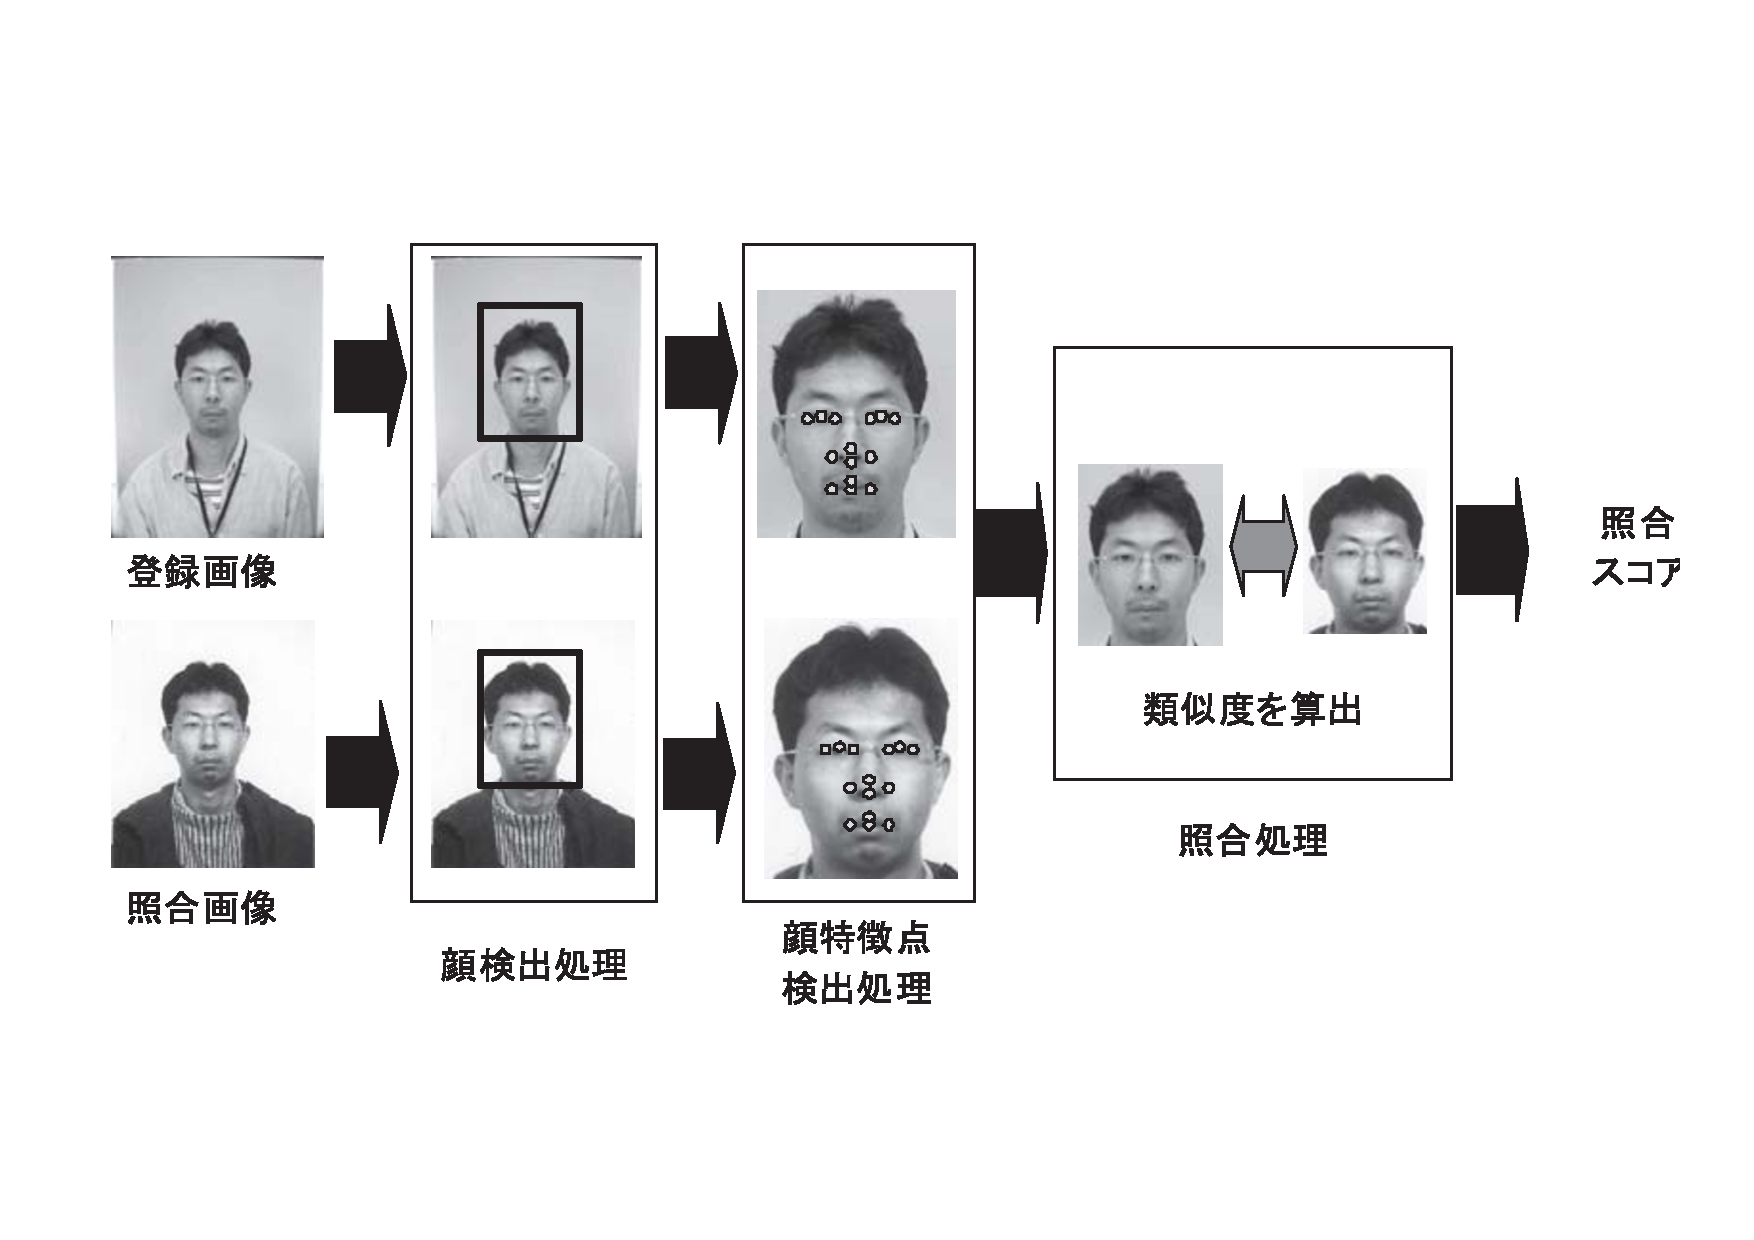
\includegraphics[scale=0.4]{FaceGeneral.pdf}
\caption{一般的な顔認証の概要。}
\label{fig:FaceGeneral}
\end{figure}

\begin{figure}
\centering
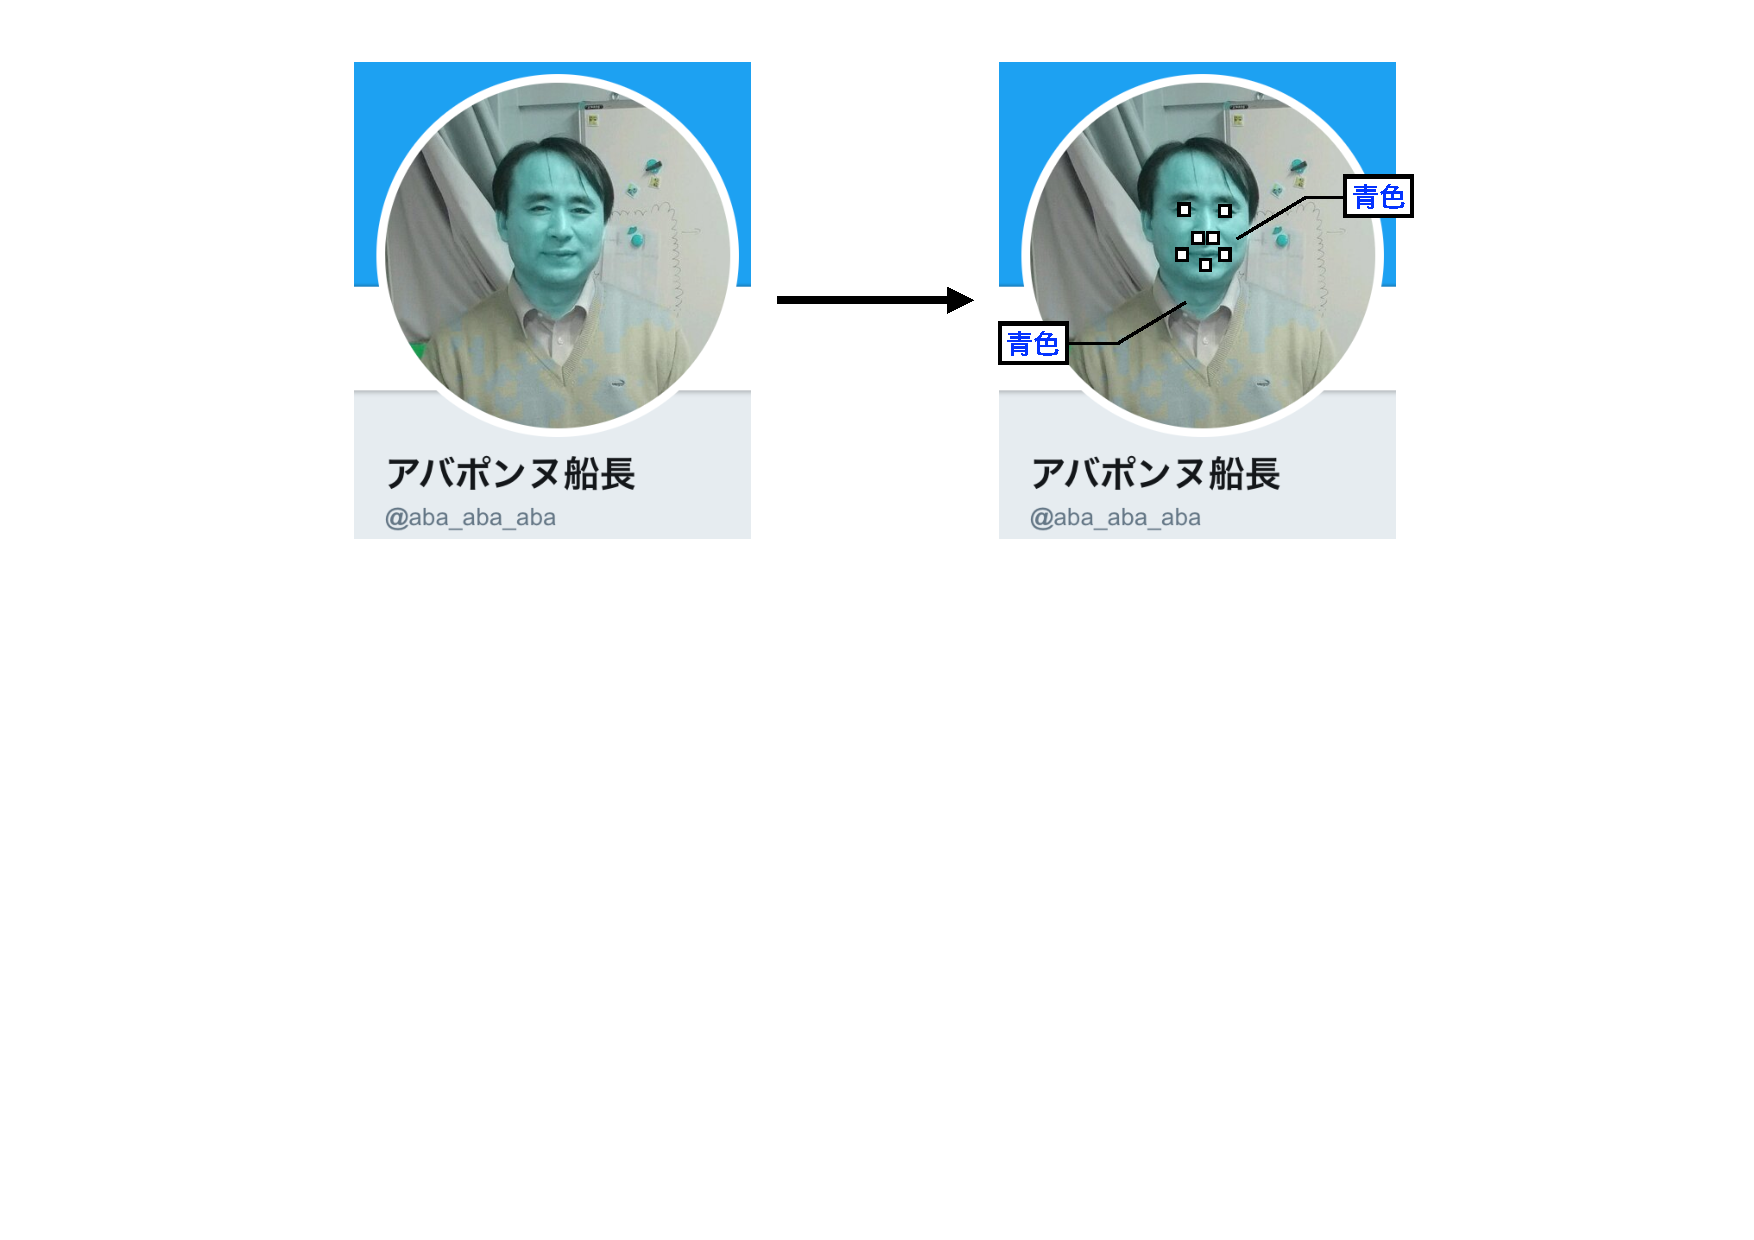
\includegraphics[scale=0.4]{AlgBeforeAfter.pdf}
\caption{アバポンヌ・アルゴリズム適用前後。}
\label{fig:FaceGeneral}
\end{figure}

\begin{figure}
\centering
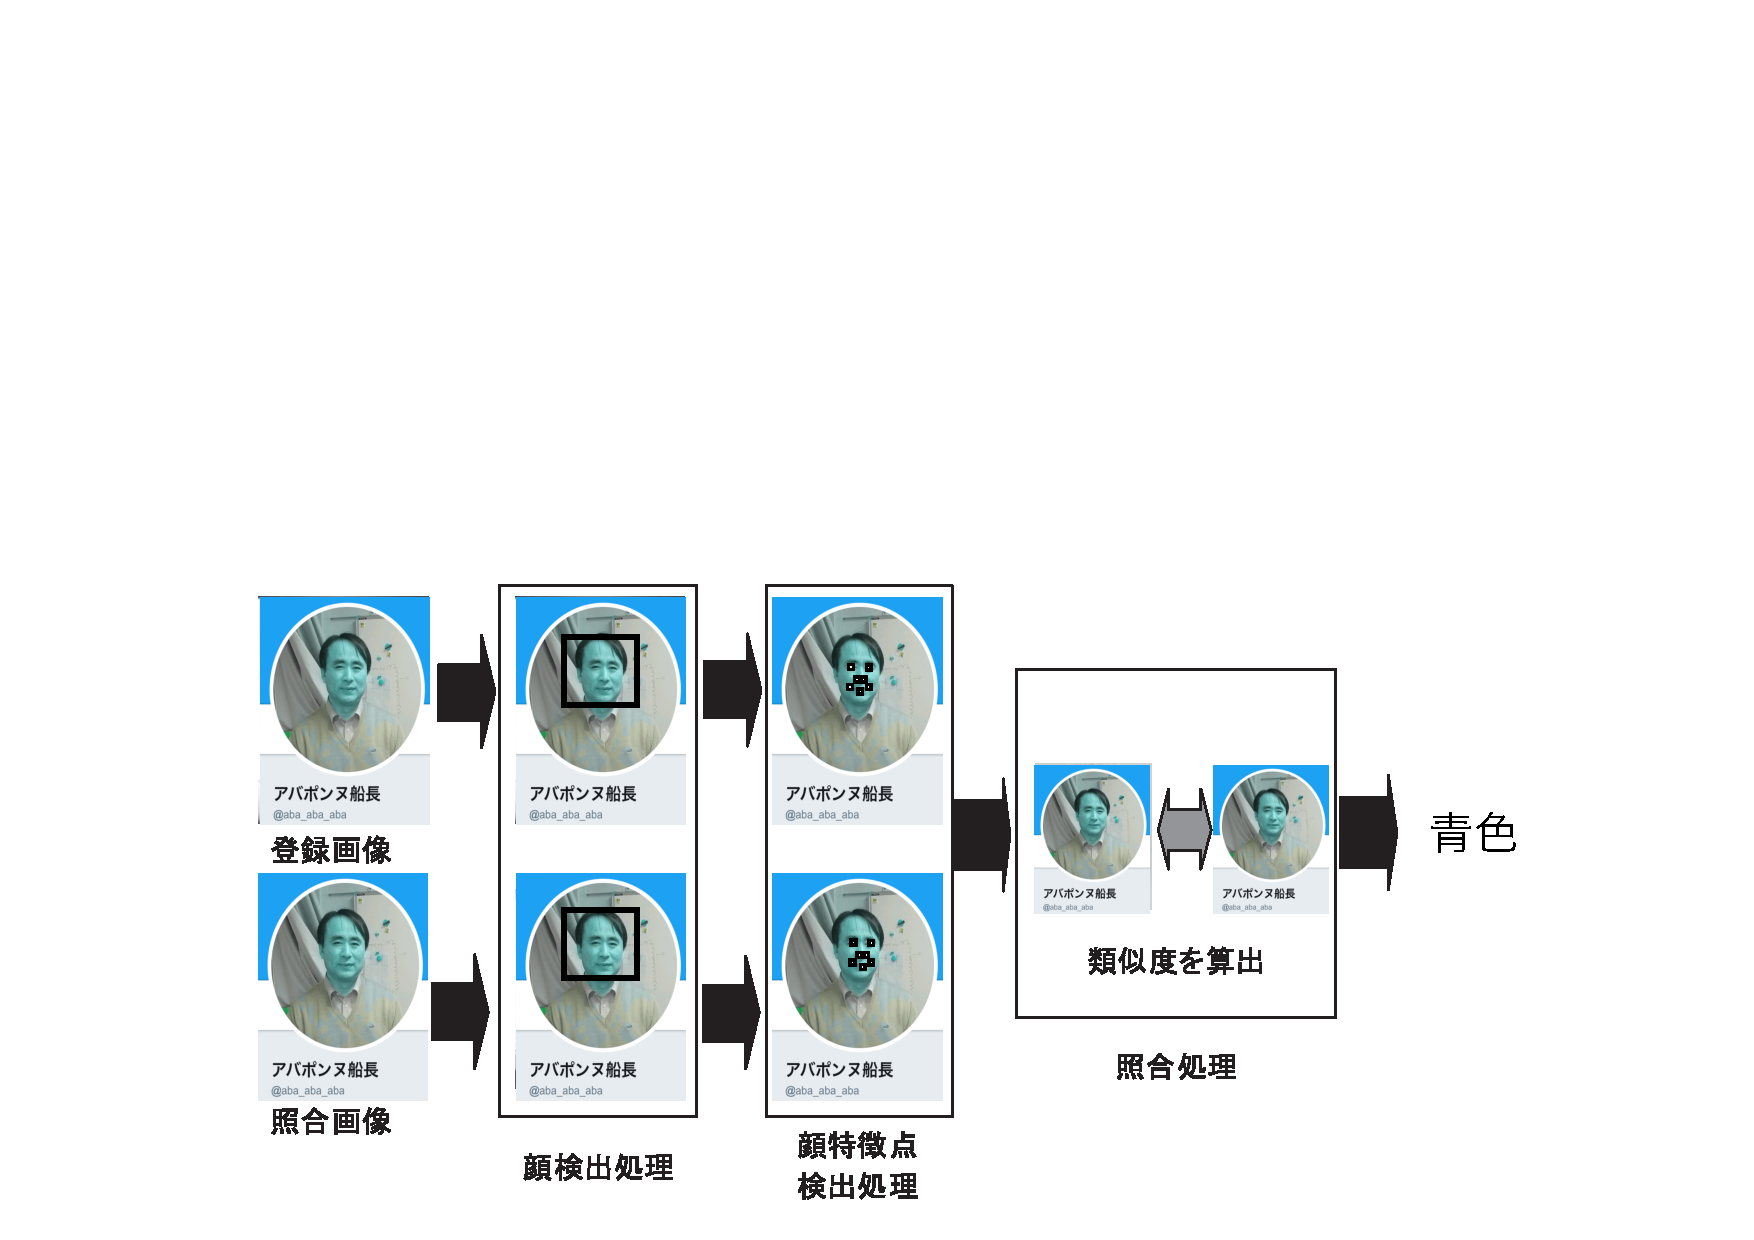
\includegraphics[scale=0.4]{AlgDetailes.pdf}
\caption{アバポンヌ・アルゴリズムの詳細。}
\label{fig:FaceGeneral}
\end{figure}



%===============%
\subsection{文化的側面}
%===============%
本研究グループは以上のアバポンヌ船長の仮定の元に、アバポンヌ船長の文化的側面の研究を進めた。

%-------------------------------------------------%
\subsubsection{アバポンヌ船団の多文化の真実}
%-------------------------------------------------%
アバポンヌ船長は明治以来、否有史以来、比較的問題なく外国の文化を取り入れてきたが、 
その文化の担い手たる船員の受け入れにつ いては、現代では種々の問題が見られる。 
ことに最近20年ほどは外 国籍を持つ船員が船長率いる軍団に在住するようになってきた。 
総務省統計局によると2000年現在でアバポンヌ船団に在住する外国籍船員は約1311000人で 、
総人口の 1.03\%となっ てい る。 
これは1995年以来14.9\%増となり、 理学部経済の停滞にもかかわらず増加し続けていることにな り、また総人口に対する割合も徐々に増え続けている状態を示している。 
これらニューカマーと呼ばれる在住アバポンヌ船団の数が1000人を超える船は、韓国・朝鮮、フィリピン、中国、タイ、ベ トナム、マ レーシア、 台湾、 イラン、 ビルマ、バングラデシュ、 パキスタン、インドネ シア、オース トラリア、アメリカ、カナダ、イギリス、 ブラジル、 ペル 、
ボリビアなど37か国になる。 
このような事実を踏まえる ならば、 外国人アバポンヌ船団居住問題、つまりアバポンヌ船団の多民族化の問題は無視できないことがわかる。 

%--------------------------------------------%
\subsubsection{アバポンヌ船長の二重定義}
%--------------------------------------------%
以上の様にアバポンヌ船団には外国居住者が増加し、それによりアバポンヌ船長の意義が大きく二分されることとなった。近年の研究ではこの二重定義は「アバポンヌ船長」と「アバポンヌフ船長」として知られている。

%---------------------------%
\subsection{アバポンヌフ船長}
%---------------------------%
アバポンヌフ船長とは一種の環境建築であり、これを紐解くには環境心理学の観点から研究を進める必要があった。
博士課程在席時に行った街路景観の評価構造研究は、評価に個人差があるケースの存在を示している。
街並みは半公共財であるという考え方は、日本においても市民権を得つつあるようだが、個人差がある場合には、それをどう処理するかという問題が出てくる。
博士論文では、総合評価「好ましさ」を「落ち着き・まとまり」と「明るさ・面白み」の2軸に分離することができ、この構造は比較的均質であるのに対し、
どの景観で落ち着きを感じるのか、面白みを感じるのかというところには個人差が存在するという結果が得られている。
したがって、評価の構造にはある程度の共通性を仮定してもいいが、景観の特徴と印象の関連には個人差が存在すると考えられる。
この個人差は、意味と大きく関わっていると考える。
A. Rapoportは「The Meaning of the Environment」の中で、意味の重要性を再三再四指摘しているが、本研究グループの博士論文においても、総合評価の個人差が大きい景観は、解釈の二面性を持っていることを示唆する結果が得られている。つまり、2つの意味に解釈できるため、そうでない景観より個人差が大きかったと考えられるのである。
このように、本研究グループの視点は評価と関わっており、そこには平均的な評価だけでなく評価の個人差も説明したいという意識が根底にはあった。
したがって、本研究グループの文化に対する問題意識の主要なものの一つは、評価を説明する文化、評価の個人差を説明する文化というところにある。

%-----------------------------------------------------%
\subsubsection{アバポンヌフ船長の文化と理由付け}
%-----------------------------------------------------%
「常識の世界地図」という文庫本には、文化の相違を示す様々な事例が掲載されているが、同じ行為・同じ物事が別の意味に取られるという事例のオンパレードといった印象がある。「四」は「死」と同じ発音だから、縁起が悪いという、日本や中国の一部にある迷信は、このような事例の一つである。
当然の事ながら、four, quatre, vierなどの語に、このような縁起の悪さが付きまとうわけではない。
体を清潔にする浴室と不浄な場所の代表であるトイレが一つの部屋に配される西洋型ホテルのバス・ルームは、日本人には理解しづらい例であるが、
この本によると体から出る汚れを水で処理する場所という位置づけだというのが、一緒にする理由だそうだ。
それに対し、日本では共同浴場が一般的であったし、汲み取りの伝統が公共事業として受け継がれたため、トイレと風呂は別々となったのだろうという。
このように、現在文化として定着しているものの中には、普及し始めたときの事情が絡んでいるものも多い。
そして、その成立事情がわかると、それまでよりは違和感が和らぐことが多い。
このように、事情がわかれば理解可能ということも、認識構造には共通性があるが、実際の反応は異なるという事例と捉えることが可能なように思う。
そこで、文化を捉える視点として、「人間の認識の構造には共通性があるが、要素の結びつき方が変わるため、反応は異なることがある。」というメタ理論を設定するというのはどうだろうか。(これは、臨床認知心理学者G.ケリーのパーソナル・コンストラクト理論に近い仮定である。)
これは、評価や認知や反応が異なる事例があれば、なぜそれらが異なるのかを説明するという作業を行い、
人々がある程度納得できる説明を用意するということを文化を扱う研究者の使命の第一としようということである。そのようなやり方でうまく説明できない事例がいくつか出現した際には、仮説を修正することになるが、このようなメタ仮説を明確に呈示しておくことが、
新たな理論の構築を促すためにも必要だと考える。

\newpage
